

\begin{lead}
 本章では,ディジタル信号処理を学ぶにあたって,
\begin{enumerate}
\item ディジタル信号処理とは何か
\item 雑音の除去
\item 画像における階調濃度の変換
\item 画像における輪郭の尖鋭化
\item 画像の符号化
\end{enumerate}
の観点からどのように実用に供しているかを説明するとともに,
実際にどのようなことを学んでおく必要があるかを概説する.

%\end{nerai}

\vfill

%\begin{koumoku}
%アナログフィルタ\\
%ディジタルフィルタ\\
%IIRフィルタ\\
%FIRフィルタ\\
%\end{koumoku}

\end{lead}


\chapter{ディジタル信号処理とは}

\label{chapter:intro}

\section{ディジタル信号処理とは何か}

本書で扱うディジタル信号とは,信号をディジタル化したもの,すなわち,信号のとり得る値が0と1のような離散的な値で表現したものであるとともに,時間方向では1秒間に一定回数で標本化した信号のことである.

そもそもディジタル信号処理とは,身近なところでいえば,

\begin{enumerate}
\item 音声処理
\begin{itemize}
\item 雑音の除去(ノイズキャンセリングなど)
\item 話者認識(音声からのテキスト生成)
\item 音声合成(テキストからの音声生成)
\item 音質の変換(ボイスチェンジャーなど)
\item 符号化(情報量の削減)
\end{itemize}
\item 画像処理
\begin{itemize}
\item 雑音の除去(ごま塩雑音やしみやしわの低減)
\item エッジ強調(輪郭抽出のようなパターン認識を行うための前処理)
\item パターン認識(形状などを判別)
\item 階調濃度の変換(プリンタへの表示)
\item 符号化(情報量の削減)
\end{itemize}
\item アナログ信号とディジタル信号との相互変換
\end{enumerate}
などのように列挙されるところである.このような手法については,信号処理とかディジタル信号処理など標榜される科目の枠組みにおいて修得することで,その原理が理解できるようになると考えられる.

本章においては,雑音の除去,画像における階調濃度の変換,画像における輪郭の尖鋭化,画像の符号化を例に概説しながら,科目修得への関連についても説明する.

%\begin{nerai}

%\clearpage

\section{雑音の除去}

信号処理といわれるところで最も身近にある例として,\index{ざつおんのじょきょ@雑音の除去}雑音の除去がある.
%
音声であれば,本来再生されるべき音(信号:signal)以外に,チリチリと聞こえる音や,周囲の騒音などによる音などを総称して雑音(noise)と呼ぶものとする.
%
つまり,可聴音(人間の耳に聞こえる音)は,信号と雑音との和で表される\footnotemark .
\begin{equation}
可聴音=信号(S)+雑音(N)
\end{equation}

\footnotetext{人間の可聴周波数(人間の耳で聞くことのできる周波数)は20Hz~20kHzといわれており,すべての周波数帯を聞くとはできないとされている.}

オーディオの世界では\index{のいずりだくしょん@ノイズリダクション}ノイズリダクションが高音質化に有効な一技術とされてきた.そして近年では,\index{のいずきゃんせりんぐ@ノイズキャンセリング}ノイズキャンセリング技術が実用に供するようになり,ヘッドフォンにノイズキャンセリングが実装されるといわれる製品も存在する.

ここで,ノイズキャンセリングの原理について概説する.

図\ref{fig:00-01}に示すように,実際に耳へ聞こえてくる音があり,雑音は周囲から発生すると仮定する.このとき,周囲からの雑音をマイクで拾い,耳へ聞こえてくる音に対して,マイクで拾った雑音を差し引くことができれば,ノイズのない音をヘッドフォンから聴くことができると考えられる\footnotemark .

\footnotetext{この説明はあくまでも平易に説明することに主眼を置いているので,厳密性はない.}

\begin{figure}[H]
\begin{center}
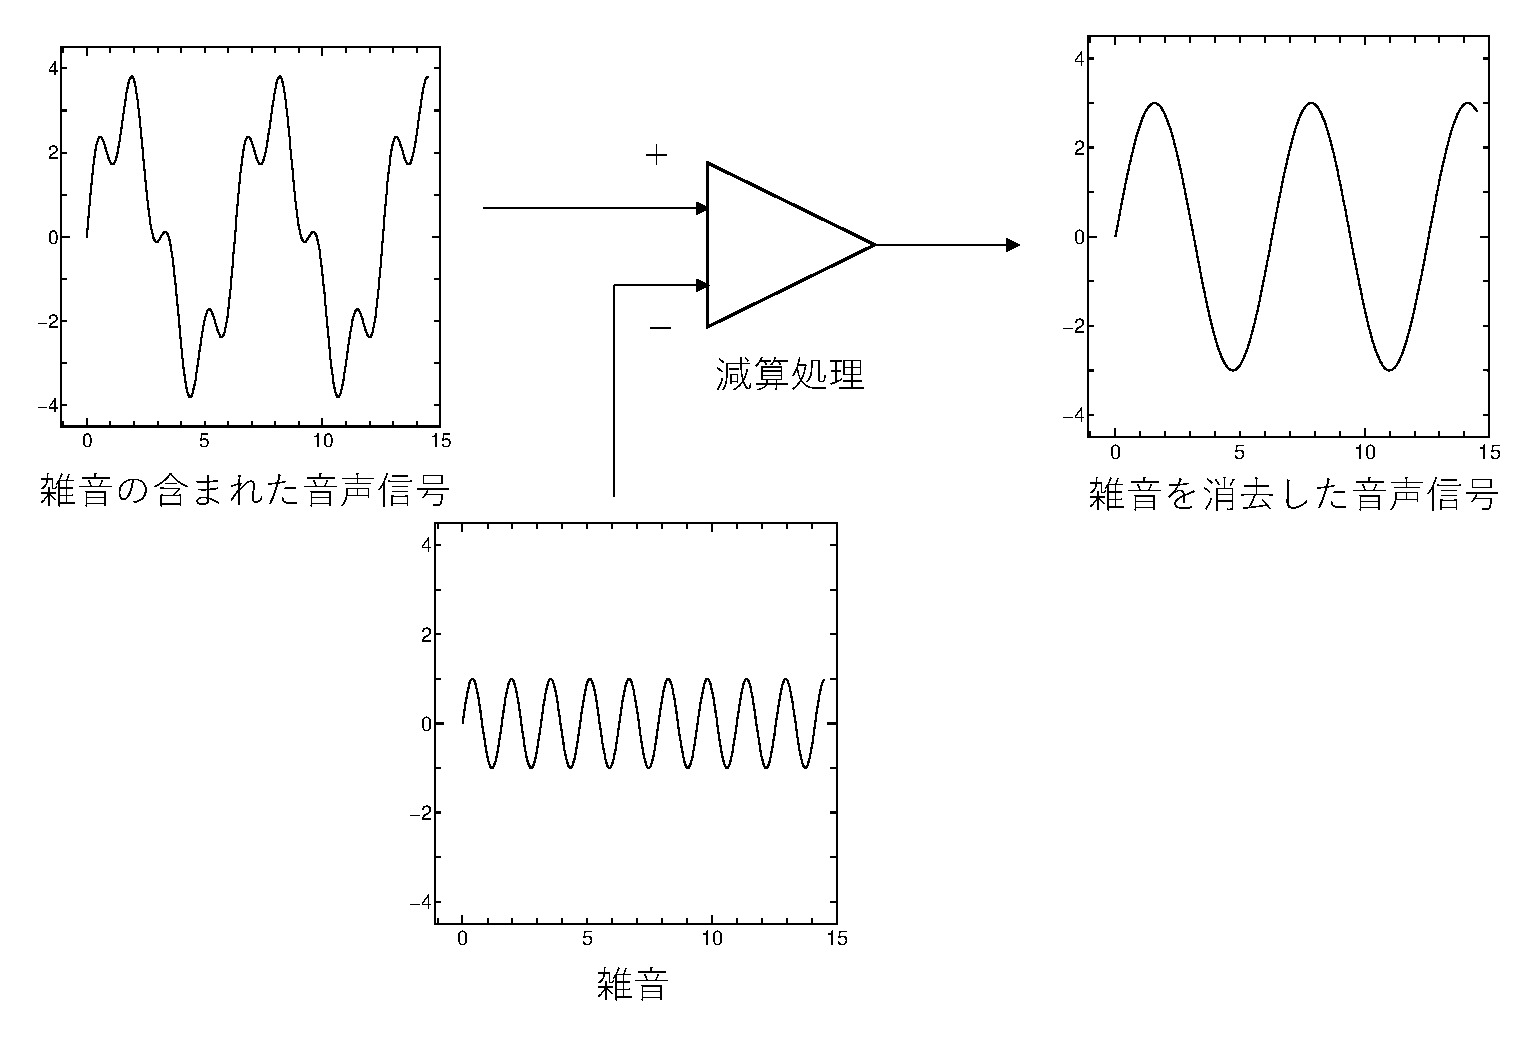
\includegraphics[width=.85\textwidth]{fig/zu-01-01.eps}
\end{center}
\caption{ノイズキャンセリングの概念}
\label{fig:00-01}
\end{figure}

ここでは,正弦波の加え合わせという考え方で原理を示したが,この原理をしっかりと理解するためには,少なくとも三角関数についての知識が必要である.また,図\ref{fig:00-01}に示すような減算処理については,電子回路における演算増幅器(オペアンプ)の原理を理解する必要もあるだろう.

ところで,先述の信号は正弦波をベースとした連続的な波形の信号,すなわちアナログ信号であった.一方,本書で扱うディジタル信号処理とは,図\ref{fig:00-02}(b)に示すような不連続点を含む信号すなわちディジタル信号を扱った信号処理である.

そこで,この図\ref{fig:00-01}に示すような原理をディジタル信号に置き換えて考えるものとする.ここでは時間軸(グラフの横軸に相当する軸)にサンプリングした信号を扱うものとする.

\begin{figure}[t]
\begin{center}
\begin{minipage}{.4\textwidth}
\begin{center}
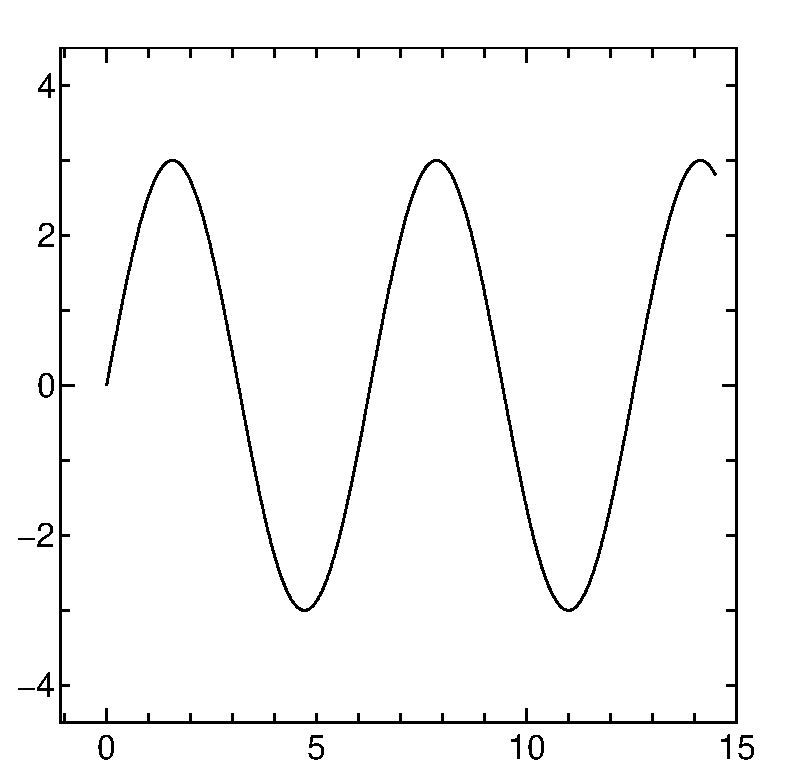
\includegraphics[width=.85\textwidth]{fig/zu-01-02a.eps}

(a) アナログ信号の例
\end{center}
\end{minipage}
\begin{minipage}{.4\textwidth}
\begin{center}
\includegraphics[width=.85\textwidth]{fig/zu-01-02d.eps}

(b) ディジタル信号の例
\end{center}
\end{minipage}\vskip.5\baselineskip
\end{center}
\caption{アナログ信号とディジタル信号}
\label{fig:00-02}
\end{figure}


\index{さんぷりんぐ@サンプリング}%
サンプリング(標本化)とは,時間軸方向に一定の周期で観測された値を示してゆくことで,結果としては図\ref{fig:00-03}のようになる.このサンプリングに関しては第\ref{chapter:6}章で説明する.時間軸方向に離散的になるため,雑音は$+1$と$-1$とを交互にとることがわかる.この雑音の符号を反転させたものと雑音とを加え合わせると,図\ref{fig:00-03}の場合であれば常に0となる.この性質から,雑音成分がわかれば,それを打ち消すように加え合わせることで,雑音の除去ができることがわかる.

\begin{figure}[t]
\begin{center}
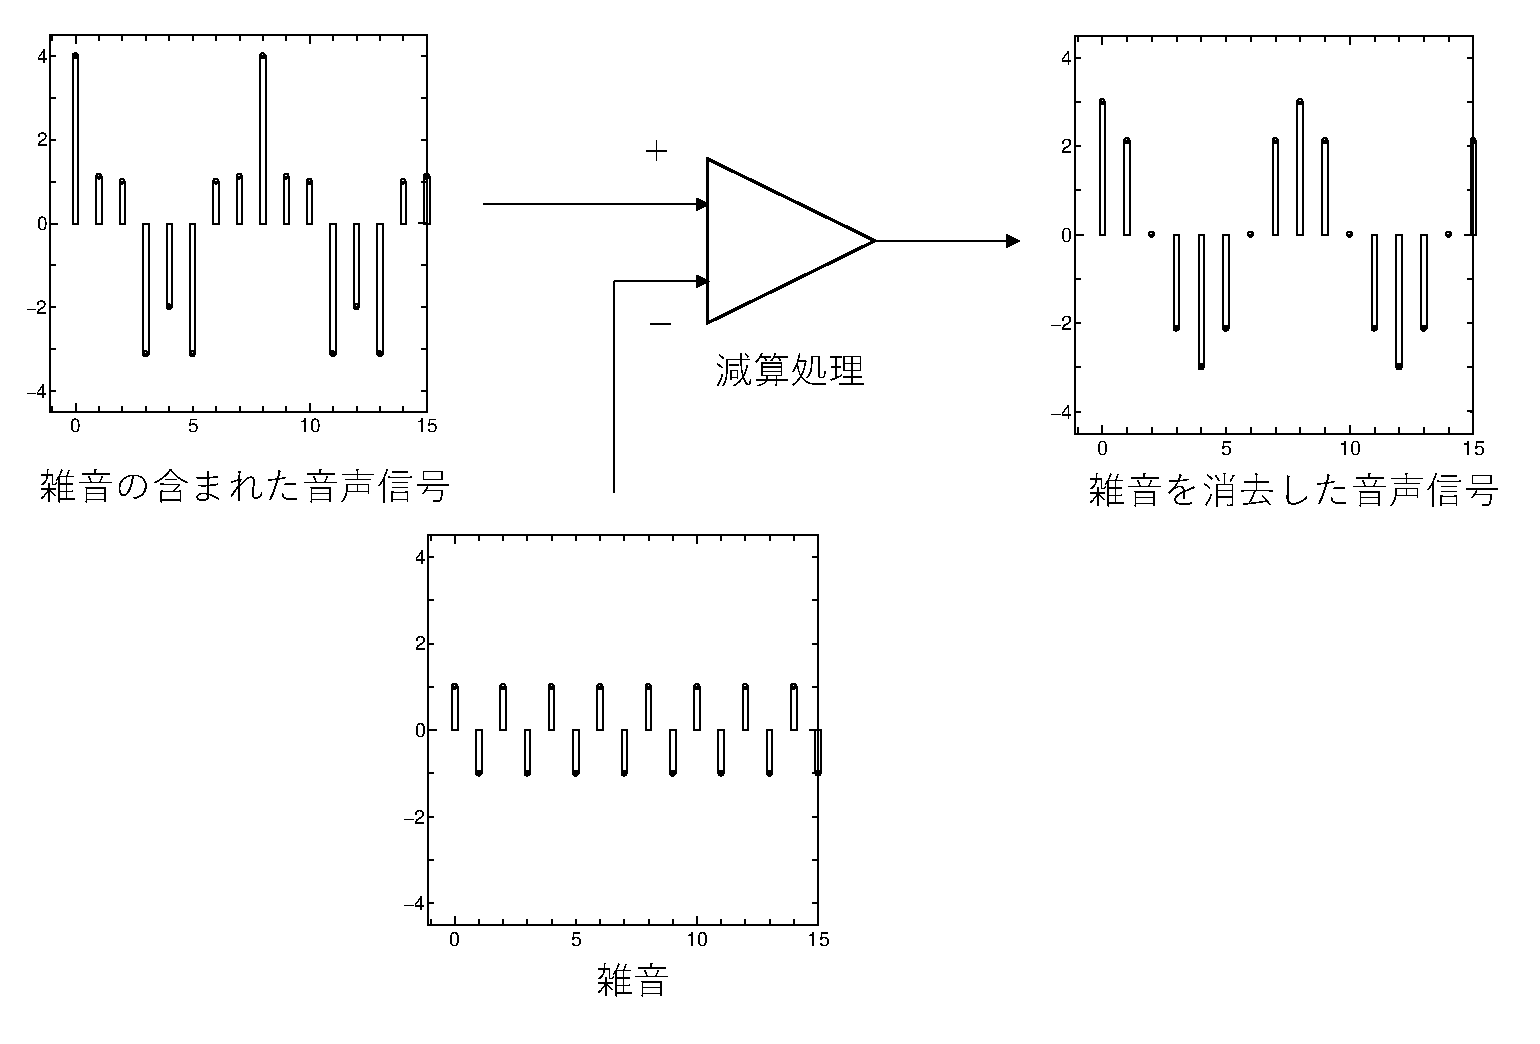
\includegraphics[width=.85\textwidth]{fig/zu-01-03.eps}
\end{center}
\caption{ノイズキャンセリングの概念(サンプリングした場合)}
\label{fig:00-03}
\end{figure}

図\ref{fig:00-04}に示すように,遅延器によって雑音の周期$T=2$の半分$T=1$なる遅延をさせ,実際の波形との加算処理を行うことによって,ひとつ前のサンプリング値との平均をとることによって,雑音の除去ができていることがわかる.

ディジタル信号処理においては,複数の時刻における信号の値を加え合わせて平均化したり,任意の組合せをしたりすることで,雑音の除去や,エッジ強調などを行うことが可能となる.このことの詳細は第\ref{chapter:ch-2}章で説明する.


\begin{figure}[H]
\begin{center}
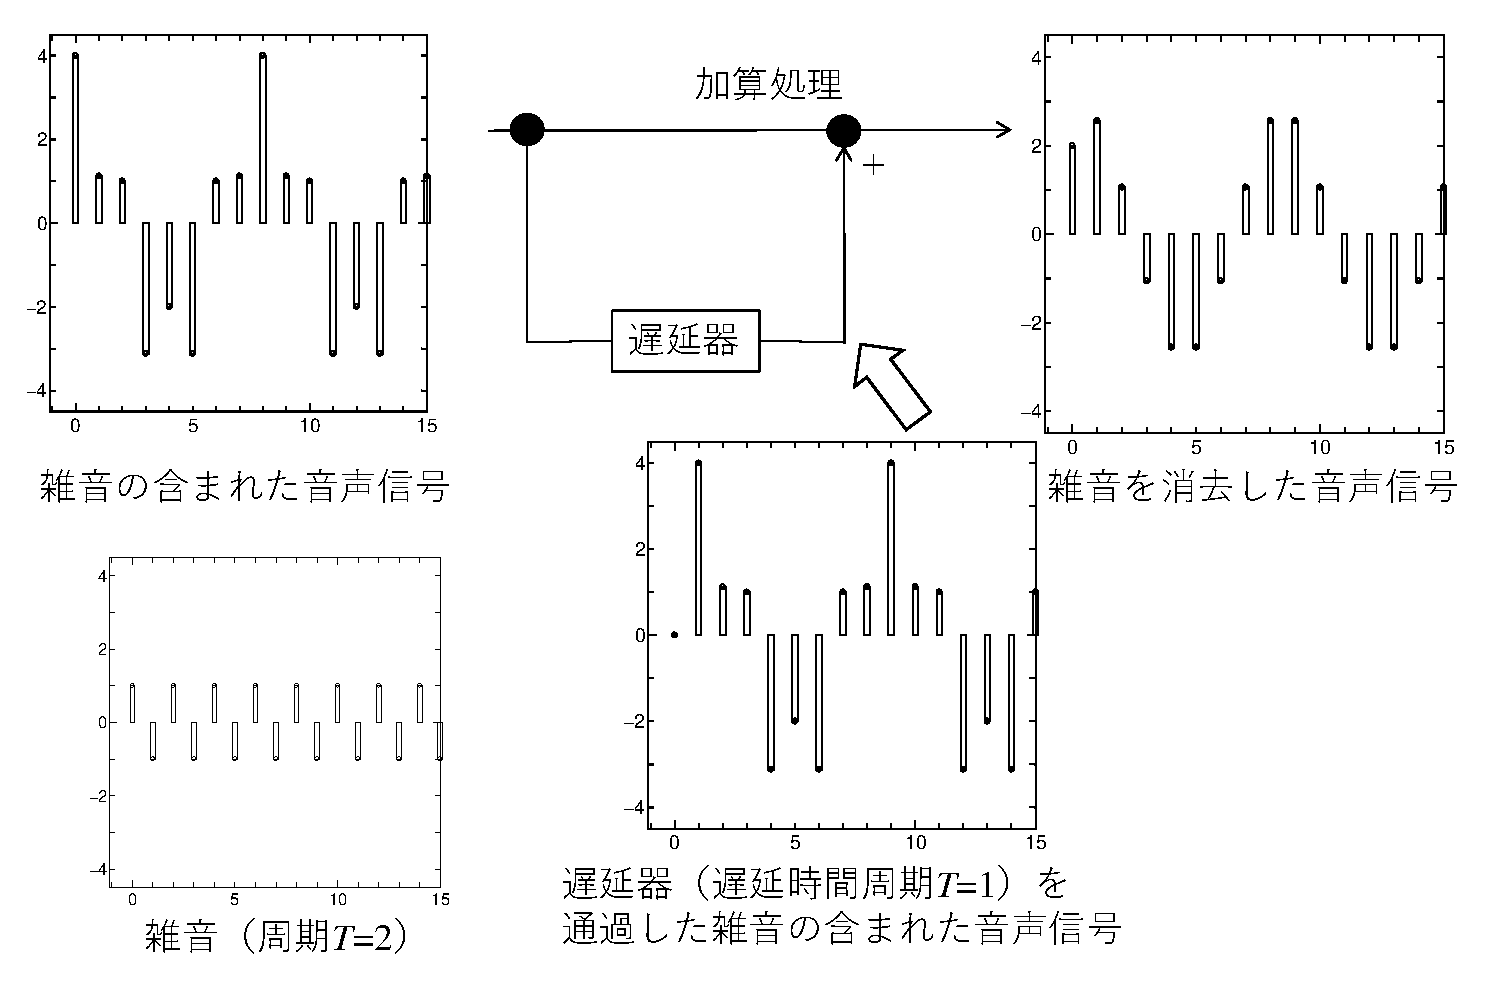
\includegraphics[width=.85\textwidth]{fig/zu-01-04.eps}
\end{center}
\caption{ノイズキャンセリングの概念(サンプリングして遅延器を用いた場合)}
\label{fig:00-04}
\end{figure}


\section{画像における階調濃度の変換}

一般的に\index{がぞうしょり@画像処理}画像処理にはさまざまな手法があるが,ここでは,概念として比較的わかりやすい,印刷のための階調数削減,\index{りんかくちゅうしゅつ@輪郭抽出}輪郭抽出,ぼかし,について説明する.

階調数削減とは,プリンタで印刷を行う際に,プリンタが持ち合わせている色(シアン:C,マゼンタ:M,イエロー:Y)で印刷可能となるようにフルカラー画像(一般的に1677万色といわれる)を8色にする処理である.また,濃淡画像(白から黒まで256階調の画像)の場合であれば白と黒の2階調に削減する処理である.

図\ref{fig:00-05}(a)は256階調の濃淡画像であり,映像情報メディア学会の``ITE標準絵柄-ヘアーバンドの女性''ある.これをプリンタで表示するために白と黒だけで構成された画像(白黒2値画像)にする.濃淡画像は256階調(0~255の整数)となっているため,各画素における階調濃度が127以下であれば0,128以上であれば255となるように2値化したものが図\ref{fig:00-05}(b)である.これだと白と黒の中間的な部分をうまく表現できていないことがわかる.そこで,図\ref{fig:00-05}(a)の原画像に周期的な雑音を重畳させて2値化したものが図\ref{fig:00-05}(c)のようなものであり,この2値化の方法をディザ法と呼ぶ.このディザ法による2値画像には輪郭の部分がぼけて見えるという問題などがあったため,図\ref{fig:00-05}(d)のような誤差拡散法による2値化を行うようになってきた.この誤差拡散法は,白か黒にする際に発生した誤差を量子化されていない画素へ繰り込む方式である.この部分において,これから学ぶ必要のある事項は,ディジタルフィルタに関する事項である.

\begin{figure}[H]
\begin{center}
\begin{minipage}{.4\textwidth}
\begin{center}
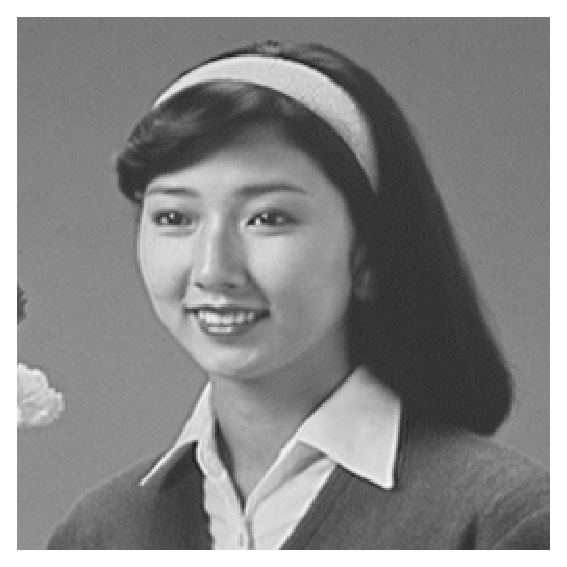
\includegraphics[width=.95\textwidth]{fig/hair1.eps}

(a) 原画像
\end{center}
\end{minipage}
\begin{minipage}{.4\textwidth}
\begin{center}
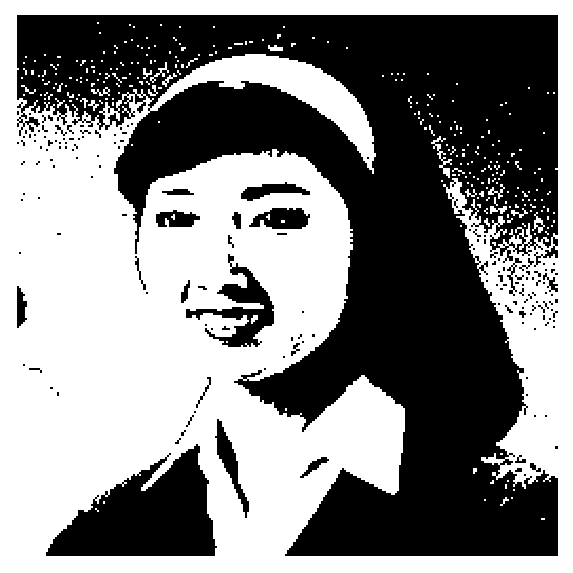
\includegraphics[width=.95\textwidth]{fig/hair1_bin.eps}

(b) 閾値(127)で白黒2値化
\end{center}
\end{minipage}
\begin{minipage}{.4\textwidth}
\begin{center}
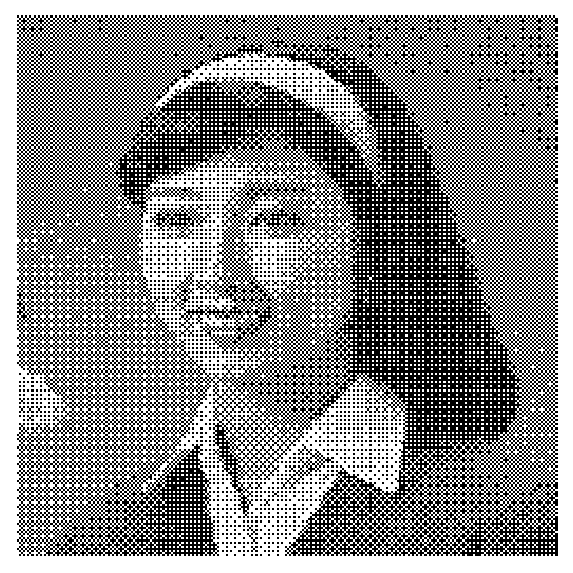
\includegraphics[width=.95\textwidth]{fig/hair1_dither.eps}

(c) ディザ法を用いた2値化
\end{center}
\end{minipage}
\begin{minipage}{.4\textwidth}
\begin{center}
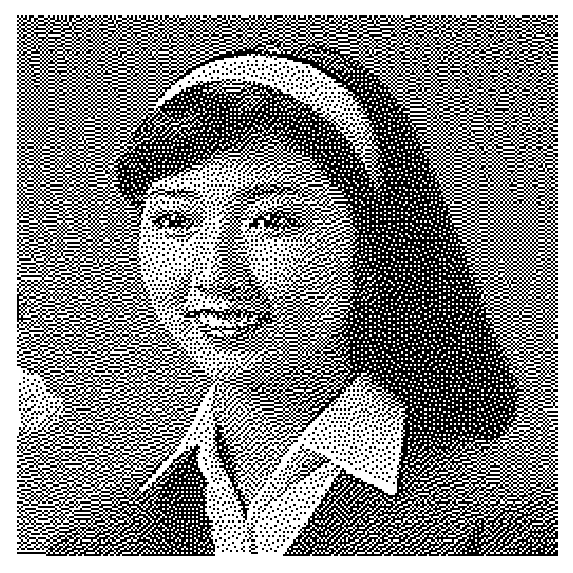
\includegraphics[width=.95\textwidth]{fig/hair1_ed.eps}

(d) 誤差拡散法による2値化
\end{center}
\end{minipage}
\end{center}\vskip.5\baselineskip
\caption{アナログ信号とディジタル信号}
\label{fig:00-05}
\end{figure}




\section{画像における輪郭の尖鋭化}

ここでは画像における輪郭の\index{せんえいか@尖鋭化}尖鋭化について概説する.この画像の尖鋭化は,少しでも輪郭を明快にすることで画質を良好にしたり,パターン認識をする際に判別しやすくしたりするための処理として用いられる.

図\ref{fig:00-07}は画像の処理として,\index{ぼかし@ぼかし}ぼかしや尖鋭化などに関する結果を示している.ここで原画像は図\ref{fig:00-05}(a)に示す映像情報メディア学会の``ITE標準絵柄-ヘアーバンドの女性''である.

図\ref{fig:00-07}(a)は画像をぼかした例である.これはしわの除去などを目的とした処理の原理となるものである.

図\ref{fig:00-07}(b)は画像のx軸方向における階調濃度変化がある部分が黒くなるようにしたものである.輪郭となる部分では階調濃度が大きく変化するので,階調濃度に関する微分をとればよいように思われるが,これでは十分な輪郭抽出がなされてるとはいえない.

図\ref{fig:00-07}(c)は画像のラプラシアン(x軸方向およびy軸方向における2階偏微分)をとったものである.この場合だと,輪郭抽出がなされているといえる.この処理をベースとした輪郭線抽出の後,パターン認識を行うという場合もある.

図\ref{fig:00-07}(d)は図\ref{fig:00-05}(a)の輪郭をシャープに見えるように処理したものである.これは図\ref{fig:00-05}(a)に図\ref{fig:00-07}(c)をあわせたものとみることができる.

\begin{figure}[t]
\begin{center}
\begin{minipage}{.4\textwidth}
\begin{center}
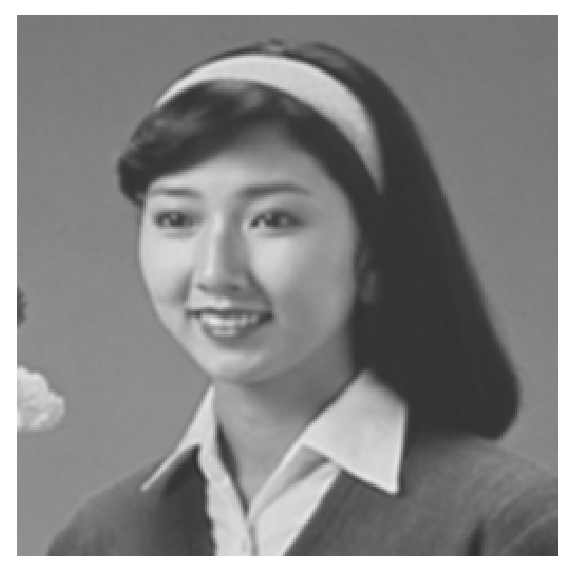
\includegraphics[width=.95\textwidth]{fig/hair1_bokashi.eps}

(a) ぼかし
\end{center}
\end{minipage}
\begin{minipage}{.4\textwidth}
\begin{center}
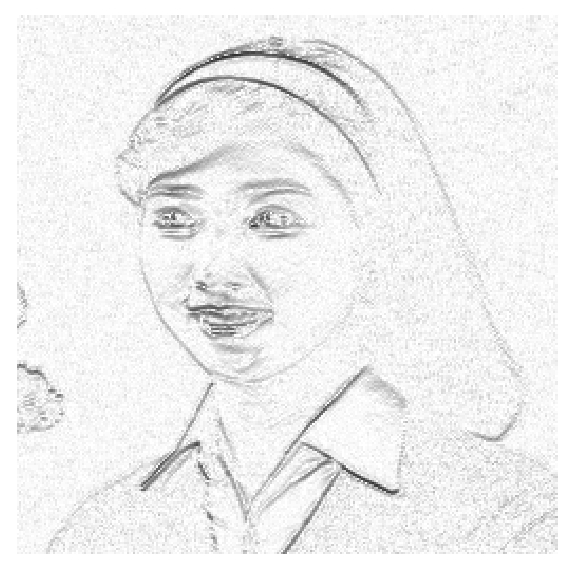
\includegraphics[width=.95\textwidth]{fig/hair1_x_sharp.eps}

(b) x軸方向に関する階調濃度の変化
\end{center}
\end{minipage}\\[.5\baselineskip]
\begin{minipage}{.4\textwidth}
\begin{center}
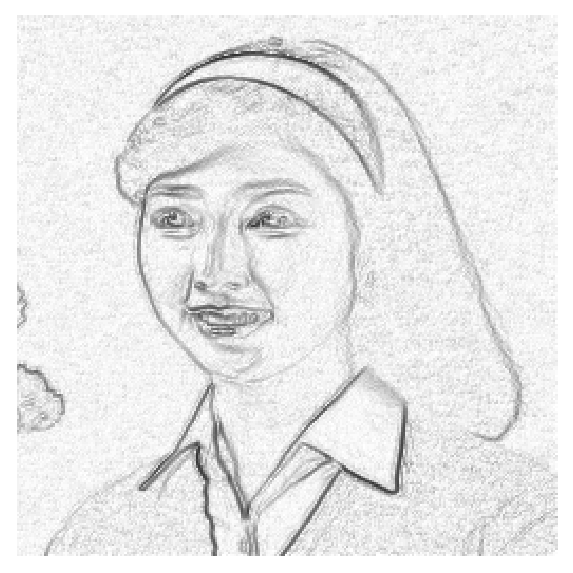
\includegraphics[width=.95\textwidth]{fig/hair1_rinkaku.eps}

(c) 輪郭流出
\end{center}
\end{minipage}
\begin{minipage}{.4\textwidth}
\begin{center}
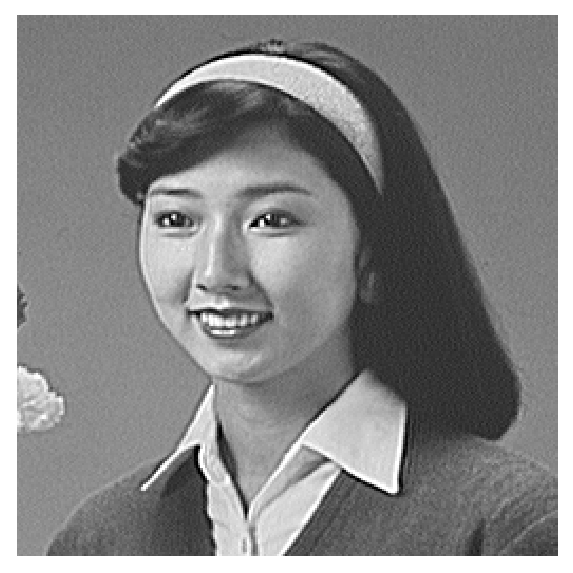
\includegraphics[width=.95\textwidth]{fig/hair1_sharp.eps}

(d) 輪郭の尖鋭化
\end{center}
\end{minipage}\vskip.5\baselineskip
\end{center}
\caption{画像処理の例(原画像は図\ref{fig:00-05}(a))}
\label{fig:00-07}
\end{figure}



このような輪郭抽出は,ぼけた画像から輪郭の部分を明瞭にするためであったり,塗り絵のための画像を生成したりするために有効とされる.またぼかしはしみやしわを除去したり,ある一定の情報が特定されないようにしたりするための処理などで用いられる.

\section{画像の\index{ふごうか@符号化}符号化}

たとえば,ディジタルカメラ,地上ディジタル放送,動画配信サービスなど課題のひとつは,それぞれの情報量の圧縮,すなわち,その情報におけるデータのサイズをいかに少なくするかということである.その成果として,高解像度でありながら高速転送が可能になるような符号化が行われ,4K放送や8K放送も試験的に行われてくるようになった.また,昨今ではアプリケーションソフトウェアのような大容量のデータについては,CD-ROMやDVDのディスク媒体に代わって,インターネットからのダウンロードによって取得するようになってきている.

実際に,これらの情報はディジタル信号すなわち0と1とが並べられているだけで構成される情報によって作られている.

アプリケーションソフトウェアについては,もともとのアプリケーションソフトウェアと同じ状態に復元できるような情報圧縮がなされる.このように圧縮後のデータから圧縮前のデータを完全復元できる符号化を可逆符号化と呼んでいる.

一方,静止画像や動画像においては人間の眼に画質劣化が感じられない程度までに情報圧縮(情報量の削減)を行っている.これを,圧縮後のデータから圧縮前のデータには完全に復元できないものの人間が得たい程度の情報は復元可能という意味で,非可逆符号化と呼んでいる.

これらのような情報圧縮技術により,通信におけるデータ量を少なくして,通信にかかるコストをできるだけ安価に抑えることができるといえる.

実際の符号化技術そのものは,情報理論といわれる科目があればそこで扱われるのだが,そのベースとなる帯域という概念(一定時間にどの程度の情報量を流通させなければならないかという指標)も知る必要がある.このためにはスペクトル解析を行う必要があるが,ディジタル信号処理というなかではフーリエ変換を用いたスペクトル解析を理解することが先決となり,それについては第\ref{chapter:dft}章~第\ref{chapter:fft}章で説明する.

また,フーリエ変換の計算は非常に複雑でコンピュータ上では大変時間の掛かるプロセスであるといわれていることから,電子回路として実装可能なように計算方式を考える必要があるとともに,できるだけ簡素で高速計算が可能な計算方式を考える必要もある.そのために開発された計算方式が高速フーリエ変換である.


\section*{演習問題}

\subsection*{問題\ref{chapter:intro}.1}

一部の画像処理アプリケーションソフトウェアにおける機能として,画像の幾何学的形状を変化させる機能がある.どのような処理を加えて機能を実現しているか考察せよ.

\subsection*{問題\ref{chapter:intro}.2}

画像の尖鋭化とぼかしについて,それぞれの長短を述べよ.

\subsection*{問題\ref{chapter:intro}.3}

\index{はいれぞりゅーしょんおーでぃお@ハイレゾリューションオーディオ}
ハイレゾリューションオーディオにおけるCDのフォーマットが44.1kHz/16bitである理由を考察せよ.

